\documentclass[12pt,a4paper]{article}

% Кодування/мови — в такому порядку
\usepackage[utf8]{inputenc}
\usepackage[T2A]{fontenc}
\usepackage[ukrainian]{babel}
\usepackage{cmap}            % коректний копіпаст з PDF (текстовий шар)
% (бажано мати шрифти cm-super у дистрибутиві)

\usepackage{geometry}
\geometry{left=2cm,right=2cm,top=2cm,bottom=2cm}

\usepackage{graphicx}
\usepackage{array,multirow,booktabs}
\usepackage{caption}
\renewcommand{\thetable}{\arabic{table}}
\captionsetup[table]{name=Таблиця}

\usepackage{amsmath}
\usepackage{pdflscape}
\usepackage{xcolor}

% Гіперпосилання — тримай наприкінці пакетів, з unicode
\usepackage[unicode]{hyperref}

\begin{document}

    \begin{titlepage}

        % Картинка шапки (по центру, з відступом від верху)
        \begin{center}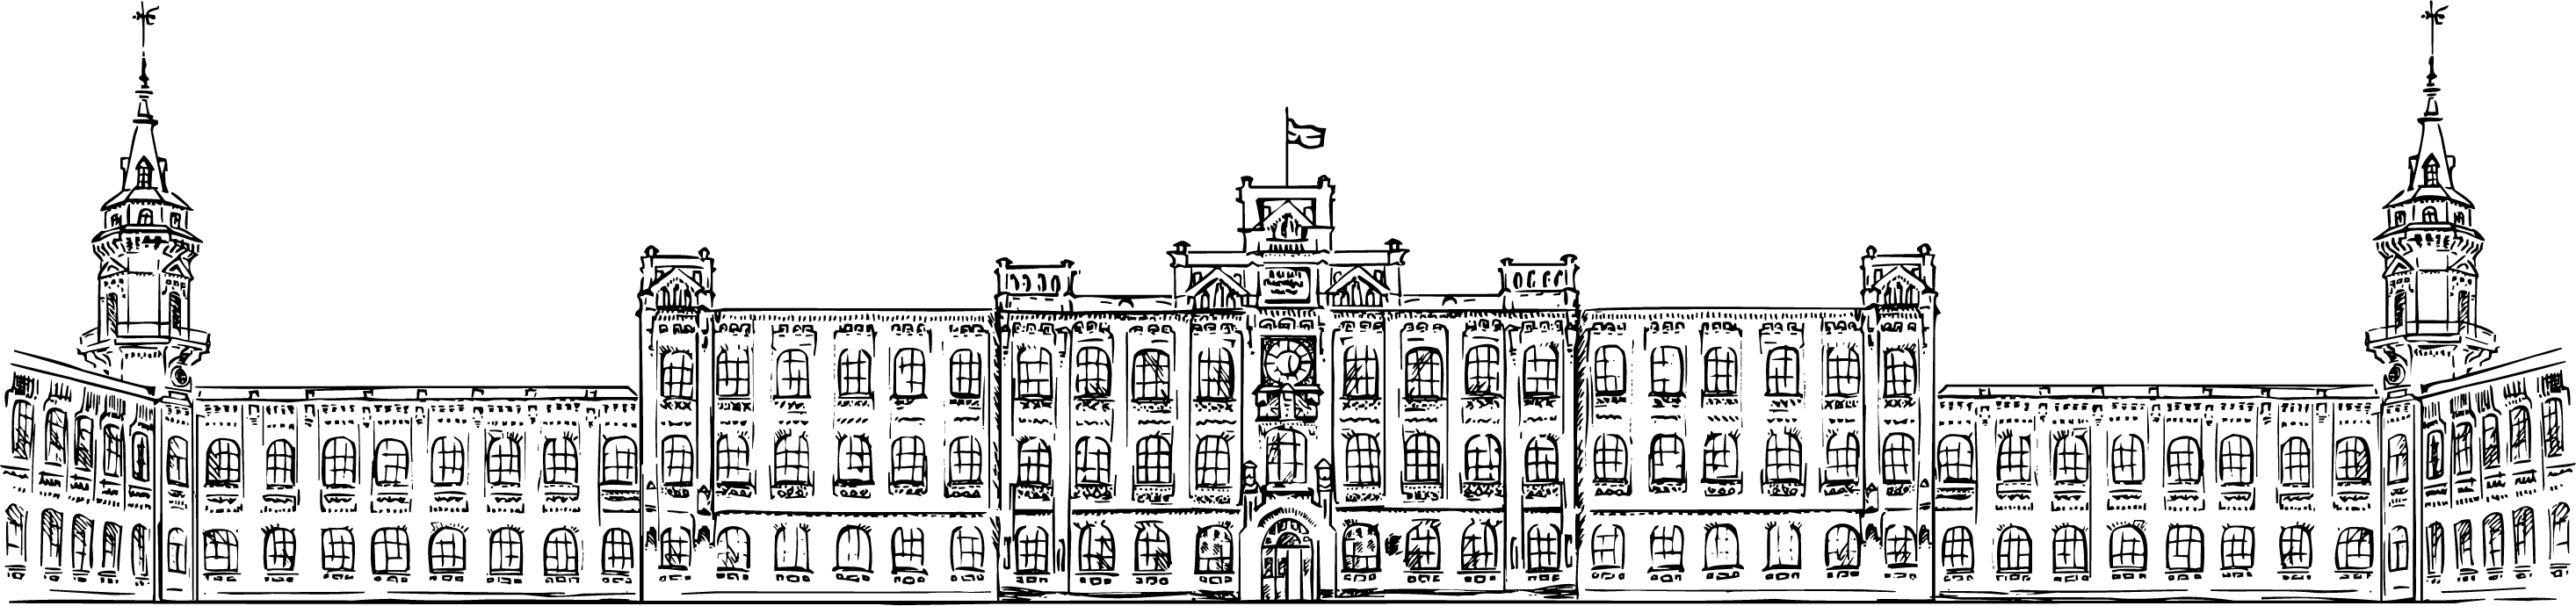
\includegraphics[width=0.7\textwidth]{../../../TITLES/letterhead.png}\end{center}

        \begin{center}
            \large Національний технічний університет України\\
            «Київський політехнічний інститут імені Ігоря Сікорського»\\[1em]
            Факультет інформатики та обчислювальної техніки\\
            Кафедра обчислювальної техніки
        \end{center}

        \vfill

        \begin{center}
            \textbf{\LARGE Теорія електричних кіл та сигналів}\\[2em]
            \textbf{\Large Лабораторна робота №2}\\
            «Використання системи комп’ютерної алгебри для дослідження математичної моделі електричного кола з використанням законів Кірхгофа»
        \end{center}

        \vfill

        \begin{flushright}
            Виконав: студент 2 курсу ФІОТ, гр. ІО-41\\
            \textit{Давидчук А.~М.}\\[1em]
            Перевірив: \textit{Лободзинський В.~Ю.}
        \end{flushright}

        \vfill

        \begin{center}Київ --- 2025\end{center}

    \end{titlepage}

    \setlength{\parindent}{0pt}

    \textbf{\underline{Тема:}} «Використання системи комп’ютерної алгебри для дослідження математичної моделі електричного кола з використанням законів Кірхгофа».

    \vspace{1em}

    \textbf{\underline{Мета:}} Навчитися використанням системи комп’ютерної алгебри для розрахунку складних електричних кіл з використанням рівнянь Кірхгофа.

    \begin{center} \textbf{\large Практична частина} \end{center}

    \setlength{\parindent}{1.5em}

    Всі розрахунки проводились за допомогою мови програмування Python (вихідний код доданий разом із звітом)

    Моя група: ІО-41, мій порядковий номер у групі: 6. Звідси $N = 6$, $S = 1$. Звідси загальна стуктурна схема електричного кола:
    \begin{figure}[h!]

        \renewcommand{\thefigure}{\arabic{figure}} % робимо "3.1", "3.2" і т.д.

        \centering
        % Підставляєте потрібний шлях та розмір зображення:
        
\includegraphics[width=0.3\textwidth]{image1.png}
        % Підпис (зазвичай під малюнком):
        \caption{}
        % Мітка для посилань у тексті (\ref{fig:...})
        \label{fig1:schema}

    \end{figure}

    Відповідно до Таблиці~1 з методичних вказівок, для $N=6$ отримуємо такі елементи у вітках (зведені у Таблиці~1):

    \begin{table}[h!]
        \centering
        \begin{tabular}{|c|c|c|c|c|c|c|}
            \hline
            Варіант & Вітка 1 & Вітка 2 & Вітка 3 & Вітка 4 & Вітка 5 & Вітка 6 \\ \hline
            6 & $R$ & $R$ & $E, R$ & $R$ & $E$ & $R$ \\ \hline
        \end{tabular}
        \caption{Елементи віток для варіанта $N=6$}
        \label{tab:myN6}
    \end{table}

    На основі елементів віток із Таблиці 1 та структурної схеми Рис. 1, побудуємо схему заміщення:
    \begin{figure}[h!]

        \renewcommand{\thefigure}{\arabic{figure}} % робимо "3.1", "3.2" і т.д.

        \centering
        % Підставляєте потрібний шлях та розмір зображення:
        \includegraphics[width=0.8\textwidth]{Figure_1.pdf}
        % Підпис (зазвичай під малюнком):
        \caption{Схема заміщення}
        % Мітка для посилань у тексті (\ref{fig:...})
        \label{fig2:schema}

    \end{figure}

    Відповідно до формул обчислення ЕРС $E_1$ та $E_2$, а також опорів $R_1$, $R_2$, $R_3$, $R_4$, $R_5$, $R_6$,
    що приведені в Таблиці 2 з методичних вказівок, отримуємо:

    \[
    E_1 = N \cdot 10, \text{В} = 60 \,\text{В}
    \]
    \[
    E_2 = N \cdot 5, \text{В} = 30 \,\text{В}
    \]
    \[
    R_1 = 50 + N \cdot S, \text{Ом} = 56 \,\text{Ом}
    \]
    \[
    R_2 = 75 + N \cdot S, \text{Ом} = 81 \,\text{Ом}
    \]
    \[
    R_3 = 120 + N \cdot S, \text{Ом} = 126 \,\text{Ом}
    \]
    \[
    R_4 = 180 + N \cdot S, \text{Ом} = 186 \,\text{Ом}
    \]
    \[
    R_5 = 200 + N \cdot S, \text{Ом} = 206 \,\text{Ом}
    \]
    \[
    R_6 = 220 + N \cdot S, \text{Ом} = 226 \,\text{Ом}
    \]

    І зводимо до зручного вигляду у таблиці:

    \begin{table}[h!]
        \centering
        \begin{tabular}{|c|c|c|c|c|c|c|c|}
            \hline
            $E_1, \text{В}$ & $E_2, \text{В}$ & $R_1, \text{Ом}$ & $R_2, \text{Ом}$ & $R_3, \text{Ом}$ & $R_4, \text{Ом}$ & $R_5, \text{Ом}$ & $R_6, \text{Ом}$ \\ \hline
            60 & 30 & 56 & 81 & 126 & 186 & 206 & 226\\ \hline
        \end{tabular}
        \caption{Розрахункові параметри ел. кола}
    \end{table}

    І на її основі побудую електричну схему в програмі Multisim:

    \begin{figure}[h!]

        \renewcommand{\thefigure}{\arabic{figure}} % робимо "3.1", "3.2" і т.д.

        \centering
        % Підставляєте потрібний шлях та розмір зображення:
        \includegraphics[width=0.8\textwidth]{test2_cropped.pdf}
        % Підпис (зазвичай під малюнком):
        \caption{Схема у програмі Multisim}
        % Мітка для посилань у тексті (\ref{fig:...})
        \label{fig3:schema}

    \end{figure}

    Запишу рівняння 2 закону Кірхгофа для всіх контурів:

    \vspace{1em}

    1 контур: $I_1R_1 + I_2R_2 = E_2$
    \vspace{1em}

    2 контур: $I_4R_4 + I_6R_6 = -E_2$
    \vspace{1em}

    3 контур: $-I_2R_2 - I_3R_3 + I_4R_4 = -E_1$
    \vspace{1em}

    А також запишу рівняння для $4-1 = 3$ вузлів I закон Кірхгофа:

    \vspace{1em}

    1 вузол: $I_5 + I_6 - I_1 = 0$

    \vspace{1em}

    2 вузол: $I_3 + I_4 - I_6 = 0$

    \vspace{1em}

    3 вузол: $I_2 - I_5 - I_4 = 0$

    Об'єднанням всих цих 6 рівнянь я отримую СЛАР:

    \[
    \left\{
    \begin{aligned}
    I_1 R_1 + I_2 R_2 &= E_2,\\
    I_4 R_4 + I_6 R_6 &= -E_2,\\
    -I_2 R_2 - I_3 R_3 + I_4 R_4 &= -E_1,\\
    I_5 + I_6 - I_1 &= 0,\\
    I_3 + I_4 - I_6 &= 0,\\
    I_2 - I_5 - I_4 &= 0.
    \end{aligned}
    \right.
    \]

    Вирішивши яку, отримуємо:

    \[
    \vec{I} =
    \begin{pmatrix}
    I_1\\ I_2\\ I_3\\ I_4\\ I_5\\ I_6
    \end{pmatrix}
    =
    \begin{pmatrix}
    0{,}364\\
    0{,}118\\
    0{,}246\\
    -0{,}208\\
    0{,}326\\
    0{,}038
    \end{pmatrix}\,A
    \]

    \begin{table}[h!]
        \centering
            \begin{tabular}{|c|c|c|c|c|c|}
            \hline
            $I_1$, А & $I_2$, А & $I_3$, А & $I_4$, А & $I_5$, А & $I_6$, А \\
            \hline
            $0{,}364$ & $0{,}118$ & $0{,}246$ & $-0{,}208$ & $0{,}326$ & $0{,}038$\\
            \hline
        \end{tabular}
        \caption{Обчисленні значення сил струмів на кожній дугі}
    \end{table}

    Значення співпадають із експериментально виміряними. Тепер складемо рівняння обчислення для потенціалів вузлів, приймаючи, що
    $\varphi_{4}=0$. Звідси: 

    \[
    \vec{\varphi} = 
    \begin{pmatrix}
    \varphi_1\\
    \varphi_2\\
    \varphi_3\\
    \varphi_4
    \end{pmatrix}
    =
    \begin{pmatrix}
    I_1 R_1\\
    E_1 - I_3 R_3\\
    - I_2 R_2\\
    0
    \end{pmatrix}
    =
    \begin{pmatrix}
    20{,}402\\
    29{,}026\\
    -9{,}598\\
    0
    \end{pmatrix}\,\text{В}
    \]

    Відповідно, обчислимо значення напруг на дугах:

    \[
    \vec{U} =
    \begin{pmatrix}
    U_{21}\\
    U_{13}\\
    U_{14}\\
    U_{32}\\
    U_{42}\\
    U_{43}
    \end{pmatrix}
    =
    \begin{pmatrix}
    \varphi_2-\varphi_1\\
    \varphi_1-\varphi_3\\
    \varphi_1-\varphi_4\\
    \varphi_3-\varphi_2\\
    \varphi_4-\varphi_2\\
    \varphi_4-\varphi_3
    \end{pmatrix}
    =
    \begin{pmatrix}
    8{,}625\\
    30{,}000\\
    20{,}402\\
    -38{,}625\\
    -29{,}026\\
    9{,}598
    \end{pmatrix}\,\text{В}
    \]

    \setlength{\parindent}{0em}

    Підведу всі результат обчислень в одну таблицю:

    \begin{table}[h!]
        \centering
        \begin{tabular}{|c|c|c|c|c|c|c|c|c|c|}
            \hline
            $\varphi_1$, В & $\varphi_2$, В & $\varphi_3$, В & $\varphi_4$, В & $U_{21}$, В & $U_{13}$, В & $U_{14}$, В & $U_{32}$, В & $U_{42}$, В & $U_{43}$, В \\
            \hline
            $20{,}402$ & $29{,}026$ & $-9{,}598$ & $0$ & $8{,}625$ & $30$ & $20{,}402$ & $-38{,}625$ & $-29{,}026$ & $9{,}598$\\
            \hline
        \end{tabular}
        \caption{Результати обчислення потенціалів та напруг}
    \end{table}
    
    \newpage
    \setlength{\parindent}{1.5em}

    Тепер перевірю правильність обчислення законом збереження енергії, або законом збереження потужності:

    \[\sum P_{\text{сп}} = \sum P_{\text{дж}}\]

    Звідси виходить:

    \[
    \vec{P}_{\text{сп}} =
    \begin{pmatrix}
    P_{1}\\
    P_{2}\\
    P_{3}\\
    P_{4}\\
    P_{6}
    \end{pmatrix}
    =
    \begin{pmatrix}
    I_{1}^{2} R_{1}\\
    I_{2}^{2} R_{2}\\
    I_{3}^{2} R_{3}\\
    I_{4}^{2} R_{4}\\
    I_{6}^{2} R_{6}
    \end{pmatrix}
    =
    \begin{pmatrix}
    7{,}433\\
    1{,}137\\
    7{,}614\\
    8{,}021\\
    0{,}329
    \end{pmatrix}\,\text{Вт}
    \]

    Звідси $P_{\text{сп}} = 7{,}433 + 1{,}137 + 7{,}614 + 8{,}021 + 0{,}329 = 24{,}534$ Вт.

    Для джерел, маємо таке:

    \[
    \displaystyle
    \vec{P}_{\text{дж}} = 
    \begin{pmatrix}
    P_{E_1}\\
    P_{E_2}
    \end{pmatrix}
    =
    \begin{pmatrix}
    E_{1} I_{3}\\
    E_{2} I_{5}
    \end{pmatrix}
    =
    \begin{pmatrix}
    14{,}760\\
    9{,}780
    \end{pmatrix}\,\text{Вт}
    \]

    \vspace{1em}

    Тут $P_{\text{дж}} = 14{,}760 + 9{,}780 = 24{,}534$ Вт.

    Звідси можемо результувати, що $P_{\text{дж}} = P_{\text{спож}}$, тобто закон збережння потужності виконується.
    Зведемо до однієї таблиці:

    \begin{table}[h]
    \centering
    \renewcommand{\arraystretch}{1.2}
    \begin{tabular}{|*{9}{c|}}
    \hline
    \multicolumn{6}{|c|}{\textbf{Потужність споживача}} &
    \multicolumn{3}{c|}{\textbf{Потужність джерела}}\\
    \hline
    $P_{1}$, Вт & $P_{2}$, Вт & $P_{3}$, Вт & $P_{4}$, Вт & $P_{6}$, Вт & $\sum P_{\text{сп}}$, Вт
    & $P_{E_1}$, Вт & $P_{E_2}$, Вт & $\sum P_{\text{дж}}$, Вт\\
    \hline
    $7{,}433$ & $1{,}137$ & $7{,}614$ & $8{,}021$ & $0{,}329$ & $24{,}534$ & $14{,}749$ & $9{,}785$ & $24{,}534$\\
    \hline
    \end{tabular}
    \end{table}

    \setlength{\parindent}{0em}

    \textbf{Висновок:} 
    На підставі розрахованих струмів $I_1,\dots,I_6$ отримано вузлові потенціали $\varphi_1,\dots,\varphi_4$
    та напруги віток $U_{ij}$. Обчислені потужності споживачів
    $P_1,P_2,P_3,P_4,P_6$ і джерел $P_{E_1},P_{E_2}$ показали виконання енергетичного балансу:
    \[
    \sum P_{\text{сп}} \approx 24{,}534~\text{Вт},\qquad
    \sum P_{\text{дж}} \approx 24{,}534~\text{Вт}.
    \]
    Отже, баланс потужностей у колі дотримано, що узгоджується із законом збереження енергії.

\end{document}